\chapter{AcCAPPCHA}\label{chapter:AcCAPPCHA}
AcCAPPCHA is a verification that works like a key-logger. This type of programs is usually malicious and intended to be used by an attacker to acquire information about the user's activity. This application analyses the sequence of keys inserted by exploiting side-channel information. Its implementation depends on the party, that the hacker wants to attack\cite{keylogging}, and that could be:
\begin{itemize}
\descItem{The user}
{these attacks are based on the exploitation of physical information related to the typing state. For example, they can use electroencephalography (EEG), motion of the wrist in the smartwatches, video with keyboard line-of-sight and WiFi signal distortion.}
\descItem{The keyboard}
{these attacks are based on analysis of signals coming from the keyboard. For example, acoustic emanations can be exploited by using external physical sensors.}
\descItem{The host}
{these attacks are based on the physical access of the attacker to the victim machine. For example, the process footprint, the CPU load and other micro-architectural analysis can be exploited in this attacks.}
\descItem{The network}
{these attacks exploit the packets exchanged in the client-server communication. For example, a network packet can be related to a keystroke revealing the key press time of the victim and the payload size of the server response.}
\end{itemize}
Analysing the previous key-logger based on side-channel information, attacks mentioned in \myref{Chapter}{chapter:SideCH} and the structure of Invisible CAPPCHA in Section \myref{Section}{chapter:InvisibleCAPPCHA}, I design this new implementation of CAPTCHA. It exploits acoustic side-channel of microphone to implement a particular type of keylogger that ensures that Authentication phase would be performed by a human user.\\
The whole implementation was created using \texttt{Python} language. The structure and the behaviour of AcCAPPCHA are similar to the ones proposed in Invisible CAPPCHA because they are both based on the evaluation of signal, detected by some sensor (motion sensors for Invisible CAPPCHA and microphone for AcCAPPCHA). With respect to Invisible CAPPCHA the program can perform also a classification of the audio signal using neural networks. The two phases of the verification are:
\begin{itemize}
\item{Evaluation of the user's activity}
\item{Communication with the remote service}
\end{itemize}
In the second phase, the username and the password of the user will be signed through ECDSA and sent by client to the authentication service if and only if the insertion was performed by a human.

\section{Evaluation of the user's activity}\label{AcCAPPCHA:user_activity}
The CAPPCHA records two audio signals: the first one created during the insertion of the password by the user and the second one created before this activity for noise evaluation. The first signal is The second signal is exploited to evaluate a noise threshold useful for the computation of amplitude peaks in the first audio.
During the insertion of the password, the instants of the time when each character was typed by the user are stored. 

\subsection{Time correspondence}\label{AcCAPPCHA:time_correspondence}
Before asking the user to insert the password, the program records an audio file of 1 second, called \texttt{noise signal}, from the built-in microphone of the laptop. The remaining verification procedure is performed by two threads simultaneously, during password insertion. The first one is continuously waiting for the insertion of a character of the password by the user until he types CARRIAGE RETURN\textit{'\r'}).\\
Immediately after a key is pressed, the time instant of this action, related to the Epoch of the PC, is stored. The sequence of time instants stored by the thread is called $x=(x_0, ..., x_{|password|-1})$. The second thread records an audio signal, called \texttt{user activity}, using the same hardware previously mentioned. This task begins its activity before the request of the password to the user and would end after the moment in which the first thread detects a CARRIAGE RETURN. Then the application removes the last 200 ms of this audio signal to be sure that the \textit{CARRIAGE RETURN} peak isn't included in recorded audio file.\\
From now on, the application has all it needs to understand if the user is a human or not. In fact the verification is performed by looking if there exists a sequence of time instants of the peaks in the signal recorded in parallel to the insertion of the password and the time instants manually stored for each character.\\
In particular \texttt{noise signal} will be analysed by finding its maximum value, called $thresh_N$, and then \texttt{user activity} will be analysed by considering only the samples with values higher than $thresh_N$. These sample will be grouped in several disjoint windows of maximum width equal to 5 ms. For each group \textit{i}, the application finds the sample with the highest value, $peak_i$. For example, given \textit{the sampling period or interval} $t_s$ and a specific group of samples: $$x_i = (x_t, x_{t+t_s}, ..., x_{t+\lceil \frac{5ms}{t_s}\rceil * t_s})$$
the application computes $t_i= argmax(x_i)$.\\
Given the sequence of computed time instants relative to peaks of each group $t=(t_0, t_1, ..., t_{n-1})$, $n$ number of windows and $|password|$ the size of the password, there is a \textbf{time correspondence} if if there exists a subset of it $t^{*}=({t*}_0, ..., {t*}_{|password|-1})$ that matches with the sequence of time instants stored during the password insertion. The algorithm used to find a time correspondence is reported next:
\begin{algorithm}[h]
\DontPrintSemicolon\footnotesize
\KwIn {$\mathtt{x =(x_0, x_1,..., x_{|password|-1})=}$ time instants stored by first thread\newline
$\mathtt{t =(t_0,t_1,...,t_{n-1})=}$ time instants relative to peaks of each group\newline
$\mathtt{threshold=}$ threshold with respect to stored time instant\newline}
\KwOut {$\mathtt{true}$ if human, $\mathtt{false}$ otherwise\newline}
\BlankLine
$\mathtt{y =(y_0, y_1,..., y_{|password|-1})}$ where $y_i=x_i-x_0$\;
\BlankLine
\If{$n<|password|$}{
\textcolor{blue}{\emph{\\Number of found peaks lower than number of characters of the password}}\;
    \BlankLine
    \Return $false$\;
    \BlankLine
}
\BlankLine
\textcolor{blue}{\emph{//Search of subsequence}}\;
\For{$i\leftarrow 0$ \KwTo $n-1$}{
\BlankLine
 \If{$(n-i)<|password|$}{
 \textcolor{green}{\emph{//Not enough peaks from $t_i$ on to be analysed to find the time correspondence}}\;
    \BlankLine
    \Return $false$\;
    \BlankLine
 }
 \BlankLine
 \textcolor{red}{\emph{//$t_i$ already verified}}\;
 $\mathtt{j\gets} i+1$\;
 $\mathtt{count\gets} 1$\;
 \BlankLine
 \While{$count < |password| \wedge j < n$}{
  \BlankLine
  \If{$(n-j)<(|password|-count)$}{
   	\textcolor{orange}{\emph{//Not enough peaks from $t_i$ on to be analysed to find the time correspondence}}\;
   \BlankLine
   $\mathtt{break}$  
   \BlankLine
  }
  \uIf{$\mathtt{(t_j-t_i)}<(y_{count}-threshold)$}{
   	\textcolor{brown}{\emph{//Too less time between the time instant of the first character and the time instant of the \textbf{count}-th character}}\;
    \BlankLine    
    $\mathtt{j}\gets j+1$\;
    \BlankLine
  }
  \uElseIf{$\mathtt{(t_j-t_i)}<(y_{count}+threshold)$}{
	\textcolor{brown}{\emph{//Time correspondence}}\;
    \BlankLine
    $\mathtt{count}\gets count+1$\;
    $\mathtt{j}\gets j+1$\;
    \BlankLine
  }
  \Else{
    \textcolor{brown}{\emph{//Too much time between the time instant of the first character and the time instant of the \textbf{count}-th character.}}\;
    \BlankLine
    $\mathtt{break}$
    \BlankLine
  }
  \BlankLine
  \If{$\mathtt{count =} |password|$}{
    \textcolor{purple}{\emph{//Time correspondence found}}\;
   \BlankLine
   \Return $true$\;
   \BlankLine
  }
  \BlankLine
 }
}
 \caption{Time correspondence}\label{AcCAPPCHA:time_algorithm}
\end{algorithm}
\clearpage
\begin{figure}[h]
     \centering
	 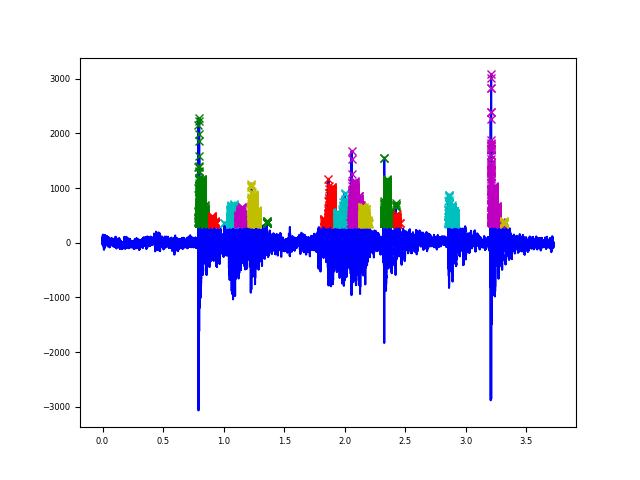
\includegraphics[width=0.8\textwidth]{Images/AcCAPPCHA/hello35_time}
     \caption{\footnotesize{Audio during insertion of password \texttt{hello35} all sub-windows highlighted.}}\label{AcCAPPCHA:hello35_time}
\end{figure}
\subsection{Character correspondence}
When pressed each key of the keyboard produces a variation of the signal, called \textit{press peak}, for a time window of about 8-10 ms\cite{keyboard_acoustic}. This signal trend can also be divided in three consecutive and distinctive areas:
\begin{itemize}
\descItem{touch peak}{peak in a window of 2-3 ms, caused by the finger touching the key}
\item{\textbf{noisy meaningless area}}
\descItem{hit peak}{peak in a window of 2-3 ms, caused by the finger and the key hitting the keyboard supporting plate.}
\end{itemize}
To obtain a prediction of each key pressed by the user, we can extract information from the touch peak, that is the most significant, and the hit peak, that increases the information related to the pression.\\
Following the idea of Asonov and Agrawal, I exploit deep learning to classify each pressed key. In the following sections, there is a detailed explanation of the main phases required and implemented for this classification method:
\begin{itemize}
\item{Data acquisition}
\item{Extraction of features}
\item{Neural network}
\item{Verification}
\end{itemize}

\subsubsection{Data acquisition}
To create a program that record audio while user type something, I created \texttt{DatasetAcquisition.py} source file containing the relative class. After instantiating an object of the class \texttt{AcquireAudio}, it applies \texttt{record} method to this instance.\\
Inside this method, two different program are run in parallel: the first one is a key-logger that is used to classify all the recorded audio files in some directories and the second one that records an audio file during keys typing. The update of private members of the class is guaranteed through the use of the mutual exclusion (mutex) management. The keylogger in the first task requires the access to the operating system signals generated by typing a key on the keyboard. It has the only purpose to continue the acquisition of the audio files even if a special key is pressed (for example F3 button).\\
The choice of running two different tasks in parallel was given by the need of recording audio before the start and after the end of password insertion by the user. Each recorded audio can contain several audio peaks related to multiple insertion of the same key but, during the acquisition of training and test set, I record one audio file for each key pressed.\\
Hence in this particular case, the key-logger waits for the insertion of a single key by the user and then reports it to the thread that performs audio recording. This last task also closes the audio stream and stores the audio signal into a \textit{wav} file named with a progressive number. All the audio files are dynamically organized into a set of subfolders of the output directory, each one with the name of the respective typed key.\\
The recording phase was performed using directly the built-in Realtek microphone and the keyboard of my MSI GL63 8RD laptop. The names of the subfolders/labels, in which each audio file of a pressed key is inserted, are reported in \myref{Appendix}{chapter:KeyMapping}.\\
Looking at Table, we can see that the keylogger changes its behaviour mapping each key to an ASCII string of upper or lower alphabetic characters because otherwise many keys would be mapped into invalid names of folders (for example, the key \textit{'.'} is now mapped into the label \textit{'POINT'}). In the table, there are two columns of labels: the first one related to the label seen by the key-logger, the second one related to the label assigned by me to each key. The reason why these labels differ for some entry are:
\begin{itemize}
\descItem{higher accuracy for spatial distribution of the keys on the keyboard}{for example, \textit{'INSERT'} and \textbf{'0\_INSERT'} (with Num lock on) would be mapped into \textit{'INSERT'} by the key-logger but they are considered different thanks to the final mapping;}
\descItem{improve the classification of keys made by key-logger}{for example, \textit{'ALT'} label is wrongly mapped into \textit{'SHIFT'} by key-logger.}
\descItem{solve the problem of keys mapped only by hardware}{\textit{FN} is the only key with this problem. The key-logger doesn't detect any pressed key, when \textit{FN} is inserted. Hence, I needed to typed it and then another key to be sure that recording for \textit{FN} was performed. Then I made another python script to resize the audio signal and remove the useless second peak.}
\end{itemize}
The last two reasons are very important because they highlight also the power of acoustic side-channel. If an attacker implements an high-level key-logger exploiting also microphone information, the accuracy of its software can increase very much.\\
In fact the hacker could collect a dataset of recordings of pressed keys on the same type of the victim's keyboard and then could train a Neural Network, that will be add in its malicious code. For each key, I record 200 audio signals obtaining a dataset of 20400 audio files. To improve the accuracy of the prediction for the neural network, I performed also Data Augmentation of the audio signals used for the training phase. I tried two approaches: 
\begin{itemize}
\descItem{Time-shift}{from each audio signal I created 4 new audio signals obtained by applying a time-shift respectively of 0.5, 1.0, 1.5 and 2.0 seconds.}
\descItem{Introduction of Gaussian noise}{from each audio signal I added a sequence of random samples from a Gaussian distribution, with standard deviation equal to 150 and mean 0, generating four new audio signals.\\
}
\end{itemize}
Using these approaches I have a training set of 2000 audio signals for key, composed respectively by the following datasets:
\begin{itemize}
\item{200 audio signals manually recorded by me}
\item{800 audio signals obtained by time-shift technique}
\item{800 audio signals from introduction of Gaussian noise}
\end{itemize}
The accuracy of the Neural Network trained on audio signals of both first and second datasets is higher than the one related to the Network trained on first dataset only.  The efficiency of the Neural Network trained on first and third dataset is worst than the one related to the network trained on first dataset only because the third dataset introduces many sequences of FFT coefficients that are very similar even if they are related to different keys. Hence I used only the network trained on the first dataset and both on the first at the second dataset as prediction model. So having 102 keys, I had respectively a dataset of 20400 and 102000 audio files.

\subsubsection{Classification}
I used three different approaches, the first two were taken from the work of Asonov and Agrawal and the last one was based on modern sound classification techniques.\\
Respectively to the method used, the feature for each key was composed by:
\begin{itemize}
\item{FFT coefficients of the touch peak}
\item{FFT coefficients of the hit peak and the touch peak}
\item{Features obtained from the hit peak and the touch peak using a deep learning pre-trained model}
\end{itemize}
In the first two cases, the coefficients are extracted from a window of 3 ms around the peaks and then they are normalized in floating point values in range $[0, 1]$ (see \myref{Figure}{AcCAPPCHA:feature_example}).\\
In the third case, the touch peak and the hit peak samples were concatenated, creating a new signal on which the spectrogram is computed (see \myref{Figure}{AcCAPPCHA:spectrogram}). From the spectrogram, I extract a feature composed by 512 values through the use of VGG16 pre-trained convolutional neural network.\\
In this way, I remove the last fully connected layers, used for classification of other task, and take the intermediate results as feature. The reason of this approach is that a pre-trained network already extracts very well features for classification of a lot of common immages and so it can extract features better than a NN created from scratch.
\begin{figure}[H]
     \centering
     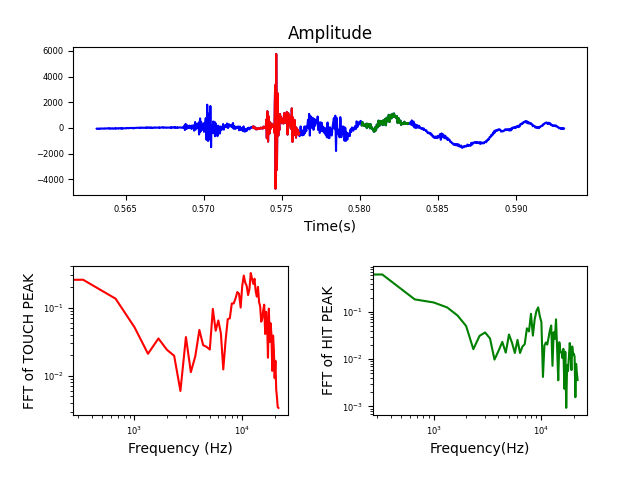
\includegraphics[width=.9\linewidth]{Images/AcCAPPCHA/feature_example}
     \caption{\footnotesize{Example of normalized FFT computation of the touch peak and the hit peak for an audio file of key \textit{'0'}.}}\label{AcCAPPCHA:feature_example}
\end{figure}
\begin{figure}[H]
     \centering
     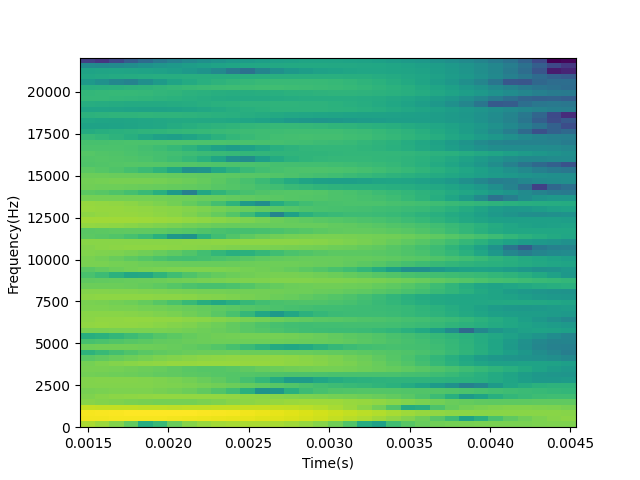
\includegraphics[width=.8\linewidth]{Images/AcCAPPCHA/spectrogram}
     \caption{\footnotesize{Example of spectrogram for an audio file of key \textit{'0'}.}}\label{AcCAPPCHA:spectrogram}
\end{figure}
\clearpage

\subsubsection{Verification}
The audio signal taken, during the insertion of the password, is analysed and then organized in windows as specified in the \myref{Section}{AcCAPPCHA:time_correspondence}, but the verification is based on:
\begin{itemize}
\item{every window previously computed}
\item{the windows that contains the time instants related to the time correspondence}
\end{itemize}
In the first approach the application uses the maximum value of each window as the touch peak and looks for the related hit peak, taking it about 10 ms after the previous peak. After the computation of the features for the two peaks, with one the methods described in the previous section, I perform the prediction using the Neural Network. I collect the most probable predicted keys and I repeat the procedure for every window initially computed on the audio. This method is very weak because after this phase, the algorithm tries to find an ordered sequence of characters, one from each window, that corresponds with the password inserted by the user. If this exists, AcCAPPCHA declares that the user was a human, otherwise a bot. The main problem of this approach is that there is no correspondence in time between a character belonging to the final sequence and the moment in which the same character was inserted physically by the user. In fact there can be false positives caused by the prediction from peak that are not related to the absolute maximum one. In other terms, in the set of the maximuma of all the windows there can be someone that is not related to the touch peak but to a local maximum.\\
The second approach solves the previous problem because the windows, where the maxima are looked for, are obtained by the correspondence time approach. In this case, AcCAPPCHA verification becomes more accurate in theory even if in practice the deep learning technique is not very efficient in prediction for a single key.

\section{Communication between client and server}
The algorithm that perform the evaluation of user activity (see \myref{Section}{AcCAPPCHA:user_activity}) is performed at client side but the value returned by it is evaluated at server-side. The response of the evaluation of user activity concatenated with a nonce and then signed through ECDSA, is sent to the server (see \myref{Section}{inv:communication}). The use of the nonce, unique and random generated sequence, is very important to guarantee that no reply attacks would be performed. In fact the server, after the reception of a message from the client, the server can check if the client has already sent the same nonce before and in this case it declines the message of the client. In this way, any attacker can't reuse a message that previously establishes a client was human. This type of procedure can be also useful to sign HTTP data, for example data sent using POST request (as insertion of password during authentication phase). In the testing phase I performed, I designed and implemented also a simplified version of the communication between the client and the server for an authentication service.\\
The application was tested on local network and the actions performed by involved parties are described in details in the following sections (see Figure ).
\begin{figure}
\centering
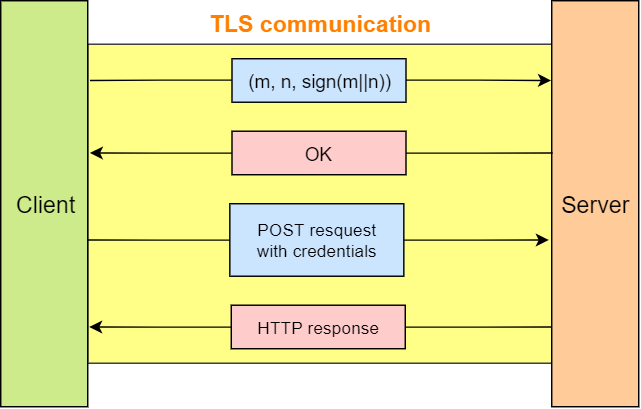
\includegraphics[width=.8\textwidth]{Images/AcCAPPCHA/client-server}
\end{figure}
\subsection{Client}
The client performs the authentication following these steps:
\begin{enumerate}
\item{It establishes a connection with the server over TLS layer to increase the security strength of the communication between the parties;}
\item{It sends the message $(m, n, sign(m||n))$ where:
\begin{itemize}
\item{$m$ is the string with the response of AcCAPPCHA algorithm on client side (\textit{'True'} if Human, \textit{False} if bot)}
\item{$n$ is the the nonce}
\item{$sign(m||n)$ is the ECDSA signature of the concatenation $m||n$ of the response and the nonce. For ECDSA was used SHA256 algorithm.}
\end{itemize}
From a practical point of view, I format the message in the following way:
\begin{table}[H]
\centering\footnotesize
\begin{tabular}{|c|}
\hline
\texttt{m CRLF n sign(m||n)}\\
\hline
\end{tabular}
\end{table}
According to basic rules in grammar of \textbf{HTTP/1.1} (see Section 2.2 of \href{https://tools.ietf.org/html/rfc2616}{RFC 2616}), \textit{CR} is the carriage return ('$\setminus r$') and LF is the line feed ('$\setminus n$'). The spaces in the message aren't considered. In this way, I can separate easily m looking at '$\setminus r\setminus n$'. The nonce has a fixed length of 16 bytes.}
\item{The client waits for response of the server with format:
\begin{table}[H]
\centering\footnotesize
\begin{tabular}{|c|}
\hline
\texttt{response CRLF}\\
\hline
\end{tabular}
\end{table}
If the answer is equal '$OK\setminus r\setminus n$', AcCAPPCHA will go on with the authentication step, otherwise the client-side application performs again the verification, asking again to user to insert the password. The maximum number of trials for a particular user is 3.}
\item{If everything goes well in the previous step, The client sends the credentials (username, password) to the server through a POST request to '/cgi-bin/auth' resource. The name of folder '/cgi-bin' comes from the standard name of the folder with functions and \textit{auth} is the name of the function that server will call. This naming approach was used very much in the past to separate functions code from pure HTML code. The password is not sent directly but it's hashed before using SHA512. The POST request used by the client has the following format:\\
\begin{table}[H]
\hspace{2cm}\centering\footnotesize
\begin{tabular}{|l|}
\hline
\texttt{POST /cgi-bin/auth HTTP/1.1} $\mathtt{\setminus r\setminus n}$\\
\texttt{Host: SP foo.example CRLF}\\
\texttt{Content-Type: SP application/x-www-form-urlencoded CRLF}\\
\texttt{Content-Length: SP SIZE CRLF CRLF}\\
\texttt{user = USERNAME $\mathtt{\&}$ pwd = HASHEDPWD}\\
\hline
\end{tabular}
\end{table}
where everything follows as before the grammar in \href{https://tools.ietf.org/html/rfc2616}{RFC 2616}). In fact also \textbf{SP} represents the space character as in the documentation. \textbf{SIZE}, \textbf{USERNAME} and \textbf{HASHEDPWD} are replaced respectively with the size of the HTTP body, the username of the client and its password hashed with SHA512.
}
\item{The client waits for the HTTP response of the server, containing HTML code as body. Then the client saves the code on the file system and opens the default web browser only to show. The HTML code is intended to show 3 possible scenarios: the user was correctly logged in, the user inserted wrong password, the username wasn't already stored on the server database.}
\end{enumerate}

\subsection{Server}
The client performs the authentication following these steps:
\begin{enumerate}
\item{It establishes a connection with the client, after his request, over TLS layer to increase the security strength of the communication between the parties;}
\item{It receives the message $(m, n, sign(m||n))$ and check the integrity of the message. To do it, the server decrypts the ECDSA signature using the client's ECDSA public key and compares the result with \textit{m||n}.}
\item{If compared messages were the same, the server checks if the nonce was already used by the same client. If so, the server thinks that there was an attacker that is performing a replay attack. If the nonce wasn't already used by the client, it will be stored in a dictionary to monitor clients activity. Each entry of the dictionary is composed by:
\begin{itemize}
\descItem{Key: IP address}{It is the IP address of the client and it is a simplification of the information that identifies a client. For example the client could be associated also to port number used to make the request, the Operating System on which the AcCAPPCHA was running on client-side or other useful parameters.}
\descItem{Value: list of nonces}{Every time a client performs a new verification request on the server, the nonce is added to the list related to its IP address in the dictionary.}
\end{itemize}
}
\item{If the nonce was used for the first time by the client, the server checks the value of the response received by the client. If the response is 'True', the server replies '$OK\setminus r\setminus n$' otherwise '$NO\setminus r\setminus n$'. If some error occurs it sends '$ERROR\setminus r\setminus n$' to the client. In the last two cases, the server terminates.}
\item{If the server doesn't terminate, it waits for the POST request from the client and analyses it to perform authentication service. The server replies to client with several status codes:
\begin{itemize}
\item{\textbf{501 (}Not implemented\textbf{)}\\
If the request is not a POST (e.g. GET)}
\item{\textbf{400 (}Bad Request\textbf{)}\\
If the number of the parameters in the POST body is different from 2 (username and password).}
\item{\textbf{200 (}OK\textbf{)}\\
If the number of the parameters in the POST body is equal to 2, the server will reply with an HTTP response with a body content depending on several cases:
\begin{itemize}
\descItem{User not in the database}{the server sends the following HTML code if the specified username isn't already stored in the database.
\begin{table}[H]
\hspace{2cm}\centering\footnotesize
\begin{tabular}{|p{6cm}|p{0.5cm}c}
\cline{1-1}
\texttt{\key{<!DOCTYPE html>}}&\multirow{7}{*}{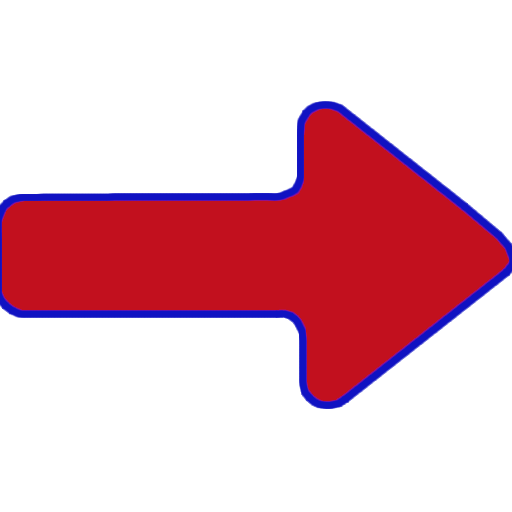
\includegraphics[width=0.5cm]{Images/arrow}}&\multirow{7}{*}{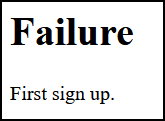
\includegraphics[scale=0.8]{Images/AcCAPPCHA/no_db_html}}\\
\texttt{\key{<html>}}&&\\
\texttt{\hspace{0.5cm}\key{<body>}}&\\
\texttt{\hspace{1.0cm}\key{<h1>}Failure\key{</h1>}}&&\\
\texttt{\hspace{1.0cm}\key{<p>}First sign up.\key{</p>}}&&\\
\texttt{\hspace{0.5cm}\key{</body>}}&&\\
\texttt{\key{</html>}}&&\\
\cline{1-1}
\end{tabular}
\end{table}
}
\descItem{Wrong password}{the server sends the following HTML code if the hashed password received from the client isn't the same with respect to the one stored in database for the specified username.
\begin{table}[H]
\hspace{2cm}\centering\footnotesize
\begin{tabular}{|p{6cm}|p{0.5cm}c}
\cline{1-1}
\texttt{\key{<!DOCTYPE html>}}&\multirow{7}{*}{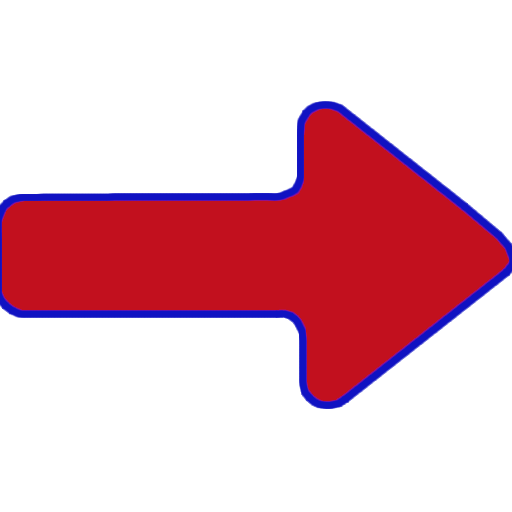
\includegraphics[width=0.5cm]{Images/arrow}}&\multirow{7}{*}{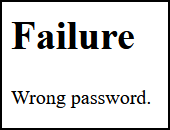
\includegraphics[scale=0.8]{Images/AcCAPPCHA/failure_html}}\\
\texttt{\key{<html>}}&&\\
\texttt{\hspace{0.5cm}\key{<body>}}&&\\
\texttt{\hspace{1.0cm}\key{<h1>}Failure\key{</h1>}}&&\\
\texttt{\hspace{1.0cm}\key{<p>}Wrong password.\key{</p>}}&&\\
\texttt{\hspace{0.5cm}\key{</body>}}&&\\
\texttt{\key{</html>}}&&\\
\cline{1-1}
\end{tabular}
\end{table}
}
\descItem{User logged in}{the server sends the following HTML code if the specified username exists in the database and  its hashed password stored in the database is the same of the one received through POST request.
\begin{table}[h]
\hspace{2.5cm}\centering\footnotesize
\begin{tabular}{|p{6cm}|p{0.5cm}c}
\cline{1-1}
\texttt{\key{<!DOCTYPE html>}}&\multirow{7}{*}{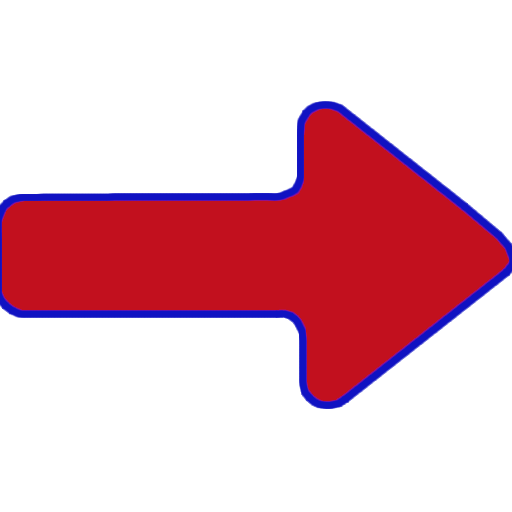
\includegraphics[width=0.5cm]{Images/arrow}}&\multirow{7}{*}{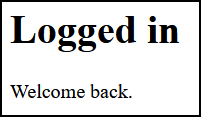
\includegraphics[scale=0.8]{Images/AcCAPPCHA/logged_html}}\\
\texttt{\key{<html>}}&&\\
\texttt{\hspace{0.5cm}\key{<body>}}&&\\
\texttt{\hspace{1.0cm}\key{<h1>}Logged in\key{</h1>}}&&\\
\texttt{\hspace{1.0cm}\key{<p>}Welcome back.\key{</p>}}&&\\
\texttt{\hspace{0.5cm}\key{</body>}}&&\\
\texttt{\key{</html>}}&&\\
\cline{1-1}
\end{tabular}
\end{table}
}
\end{itemize}
}
\end{itemize}
}
\end{enumerate}

\subsection{Database}
The database, created to simulate the search of a username by the server, was made using PostgreSQL. I could store all the information in a simple text file or a csv file but I decide to use this approach to be more flexible to future integration to more complex database.\\
The database is composed by only a table \texttt{CloudUser} to store information about user identity usually stored during the sign up phase. The creation of the database was performed through the following instructions:
\lstset{basicstyle=\footnotesize,breaklines=true}
\lstinputlisting[language=SQL]{../Code/PC/dat/db/db_creation.sql}
I created several domain to manage format of some information of the user. For example the password is a string of 128 characters because each password is hashed using SHA512 and then formatting the result as a string of hexadecimal values.
Then I populated the dataset with some entries, related to fake user, only for testing purpose. An example of inserted users is the following one:
\vspace{0.5cm}
\begin{lstlisting}[language=SQL, showstringspaces=false]
INSERT INTO CloudUser (Name,
                       Surname,
                       Username,
                       Email,
                       Sex,
                       Password)
                       
VALUES ('Raffaele', 
        'Di Nardo Di Maio', 
        'RaffaDNDM', 
        'example1@gmail.com', 
        'Male',
        HASHPASSWORD);
\end{lstlisting}
In practice, \texttt{HASHPASSWORD} is replaced by the string of 128 characters corresponding to the hashed password in hexadecimal format.

\subsection{Encryption Keys}
The creation of the TLS socket for the communication between the client and the server is done by using keys and certificates created thanks to the following bash instructions:
\vspace{0.3cm}
\begin{lstlisting}[language=bash, showstringspaces=false, tabsize=4]
openssl req -new -x509 -days 365 -nodes -out client.pem
		-keyout client.key
\end{lstlisting}
\begin{lstlisting}[language=bash, showstringspaces=false, tabsize=4]
openssl req -new -x509 -days 365 -nodes -out server.pem 
		-keyout server.key
\end{lstlisting}
OpenSSL is a open-source implementation of TLS/SSL protocols and, thanks to the option \texttt{-x509}, you can display certificates and also access to many signing protocols.
In particular, in the previous bash instructions, a X.509 Certificate Signing Request (CSR) is generated and signed for both the parties.\\
Thanks to \texttt{-nodes} the private key is created and not encrypted. The certificates are stored respectively in \textit{server.pem} for the server side and \textit{client.pem} for the client and they are valid for 365 days. The private keys are stored thanks to \texttt{-keyout} option in the \textit{client.pem} and \textit{server.key}.\\\\
The keys, used in ECDSA signing and verification, were created as follow from Python language instead of using a bash tool:
\vspace{0.3cm}
\begin{lstlisting}[language=python, showstringspaces=false, tabsize=4]
from ecdsa import *
from hashlib import sha256

PRIVATE_KEY = SigningKey.generate(curve=SECP256k1,
                                  hashfunc=sha256)

with open('ecdsa.key', 'w') as private_pem:
	private_pem.write(PRIVATE_KEY.to_pem().decode())

PUBLIC_KEY = PRIVATE_KEY.get_verifying_key()

with open('ecdsa.pem', 'w') as public_pem:
	public_pem.write(PUBLIC_KEY.to_pem().decode())
\end{lstlisting}
The \textit{ecdsa} module gives access to the management of operations performed by signing and verification phase. In this case the private key, used to sign a message from the client, was computed on the curve \texttt{SECP256k1} usually used in Bitcoin applications.